% Finished 
% Put into VUW Thesis format Wednesday 2 April 2014

\documentclass[12pt, a4paper, twoside, openright]{book}

\usepackage{vuwthesis} % sets up some local things, mostly the front page

\setlength{\intextsep}{12pt} % set space above and below in-line float
\setlength{\abovecaptionskip}{0pt} % set space between figure and caption.

\usepackage{url}

\usepackage{amssymb, amsmath}
%\usepackage{mathtools}
\usepackage{tikz}
\usetikzlibrary{calc}

\newcommand{\beff}{\ensuremath{b_{\mathrm{eff}}}}
\newcommand{\bmin}{\ensuremath{b_{\mathrm{min}}}}
\newcommand{\bmax}{\ensuremath{b_{\mathrm{max}}}}

\newcommand{\blow}{\ensuremath{b_{\mathrm{low}}}}
\newcommand{\bhigh}{\ensuremath{b_{\mathrm{high}}}}

%\usepackage{marvosym}

\usepackage{etoolbox}
\newtoggle{compilealone}
\toggletrue{compilealone}

\title{Chapter 10: Conclusion}
\author{Nat Lund}

\begin{document}
\chapter{Conclusion}\label{C:conclusion}

\section{Summary}

In this PhD thesis we studied the effective slip length of Stokes flow over rough heterogeneous surfaces.  In our mathematical model, the rough surface is modelled as a periodic function $h(x,y)$, and the local intrinsic slip length is modelled as a periodic function $b(x,y)$.  The period $L$ of both functions is the same.  The slip function $b(x,y)$ has a minimum $\bmin$ and a maximum $\bmax$.  At some height $P$ above the surface, a fixed velocity or shear rate drives the fluid.

Using the homogenization technique for partial differential equations, we showed that if $L$ is much smaller than other length scales, then the effective slip length is well-approximated by the harmonic mean of intrinsic slip lengths, weighted by area of contact between fluid and surface:

\begin{equation}
\beff = \left< \frac{\sqrt{1+ |\nabla h|^2}}{b(x,y)} \right>^{-1}
\end{equation}

%We tested this formula against a numerical simulation using finite element methods.  The FEM results show excellent agreement with our prediction:  If $L$ is 5\% of $P$, then the slip length calculated from the FEM solution is within 5\% of our predicted $\beff$.

% if $L \ll \bmin$, and are even within 5\% of our prediction when $L \sim \bmin$.

\clearpage
Using a quite different technique, a perturbation method, we replicated this result for the simplified case where the surface is flat, not rough:

\begin{equation}
\beff = \left< \frac{1}{b(x,y)} \right>^{-1}
\end{equation}

The perturbative result reconciles with the homogenized result, since for a flat surface $\sqrt{1+ |\nabla h|^2} = 1$.  The perturbative result also applies when $L$ is much smaller than other length scales.

Also using the perturbation method, we studied flat surfaces in the limit of vanishing slip length. If $\bmax \ll P$, then the slip length is expected to be best approximated by the area-weighted average of intrinsic slip lengths:
% where the length scales are in the opposite relation: $\bmax \ll L$.  In this regime, the effective slip length is simply the area-weighted average of intrinsic slip lengths:
\begin{equation}
\beff = \left< b(x,y) \right>
\end{equation}


We then tested these effective slip length formulae with numerical simulations using the finite element method.  The tests confirmed that the formula are excellent approximations in their respective limits. For example, if $L$ is 5\% of $P$, then  $ \beff = \left< \frac{1}{b} \right>^{-1} $ is within 1\% of the effective slip length calculated from the FEM simulation. The numerics also revealed that the harmonic mean formula is a surprisingly good approximation in the case where $L$ is of the same order as $b$, and both are smaller than $P$.  Finally, the numerics suggested that the simple mean formula is a good approximation only when $b$ is on the order of two orders of magnitude smaller than $L$, which itself is much smaller than $P$.

To summarise:
\begin{equation}
\text{If  } L \ll P,b: \qquad \beff \simeq \left< \frac{\sqrt{1 + |\nabla h|^2}}{b}  \right>^{-1}
\end{equation}

\begin{equation}
\text{If  } L \sim b \ll P: \qquad \beff \approx \left< \frac{\sqrt{1 + |\nabla h|^2}}{b}  \right>^{-1}
\end{equation}

\begin{equation}
\text{If  } b \ll L \ll P: \qquad \beff \simeq \left< b  \right>
\end{equation}


%\clearpage

\section{Consequences}

What are the consequences of these formulae for the engineers of, say, nanostructured superhydrophobic surfaces?

Consider a \textbf{binary} surface, composed of two different surface types, low-slip regions (eg. Teflon), and high-slip regions (eg. air gaps).  Let $\phi$ be the area fraction of the surface that is occupied the low-slip region.  
Then given fixed intrinsic slip lengths $\blow$ and $\bhigh$ for the two regions, the two effective slip expressions are:
\begin{equation}
\beff = \left< \frac{1}{b} \right>^{-1} =
\left[ \phi \frac{1}{\blow} + (1-\phi) \frac{1}{\bhigh} \right]^{-1}
\label{eq:harmbinary}
\end{equation}
and
\begin{equation}
\beff = \left< b \right> = \phi \blow + (1-\phi) \bhigh
\end{equation}


We plot the predicted effective slip lengths as a function of $\phi$ in Figure (\ref{formulaeplot}).

\begin{figure}[ht]
\centering
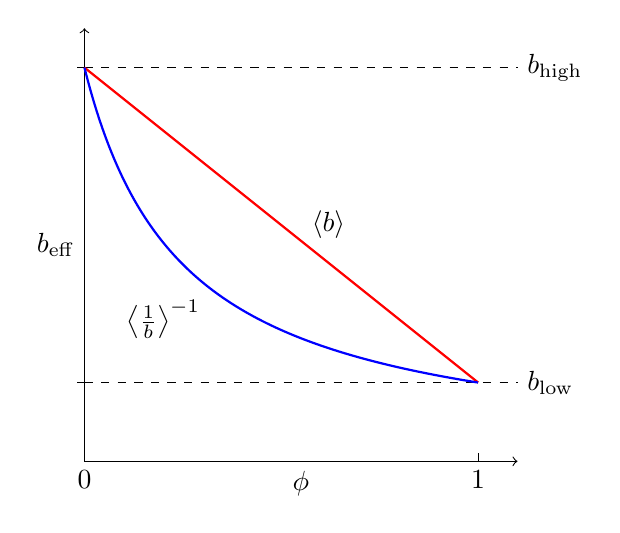
\begin{tikzpicture}

\draw[<->] (0,5.5) -- node[left]{\beff} (0,0) -- node[below]{$\phi$} (5.5,0);
\node at (0,0) [below]{0};
\node at (5,0) [below]{1};
\draw (5,0) -- ++(0,0.1);
\draw (0,1) -- ++(-0.1,0);% node [left] {\blow};
\draw (0,5) -- ++(-0.1,0);% node [left] {\bhigh};

\draw[dashed] (0,1) -- ++(5.5,0) node [right] {\blow};
\draw[dashed] (0,5) -- ++(5.5,0) node [right] {\bhigh};

\draw[thick,red] (0,5) -- (5,1);
\draw[thick,blue] [domain=0:5,samples=200] plot (\x, {1/( (\x/5) *1  + (1-(\x/5))*0.2  )} );

\node at (3.1,3) {$\left< b \right>$};
\node at (1,1.8) {$\left< \frac{1}{b} \right>^{-1}$};

\end{tikzpicture}
\caption{The harmonic mean $\beff$ formula (blue), and mean formula (red, straight), as functions of  $\phi$, for a flat binary surface where $\phi$ is the area fraction with $\blow$.}\label{formulaeplot}
\end{figure}

\clearpage
The graph of Figure (\ref{formulaeplot}) is possibly bad news for a nanoengineer aiming to maximise effective slip.  A typical nanoengineering effort may involve a nanopatterned surface, say nanogrooves, with a period of tens of nanometers, on the wall of a micron-sized pipe.  Air trapped in the nanogrooves creates a liquid-gas interface with a slip length on the order of microns.  A credible slip length for the solid surface is perhaps 20 nm (see Chapter 2). Then $L \ll P, b$ or $L \sim b \ll P$, and the harmonic mean formula of Equation (\ref{eq:harmbinary}) applies.  As Figure (\ref{formulaeplot}) shows, $\beff$ is \textbf{dominated by the lowest slip present,} and a large $\beff$ is achieved only with a very small fraction of low-slip surface.

%The graph is possibly bad news for a nanoengineer: For surface tension to support water on top of air gaps, the air gaps must be quite narrow, hence period $L$ is very small.  Then it is likely that $L < \bmin$, so the harmonic mean formula applies, and therefore, $\beff$ is \textbf{dominated by the lowest slip present.}  The lower (blue) line of the graph shows that a large $\beff$ is achieved only with a very small fraction of low-slip surface.

%Conversely, for macroscale patterning, one has $\bmax \ll L$, and so the simple mean formula applies.  In that case, any increase in the area of the high-slip region generates a proportional increase in $\beff$.


\section{Future Work}

We have mathematically rigorous results for an approximate $\beff$ that is a good approximation if $L \ll P$, and a progressively better approximation as $L/P$ gets smaller.  Assuming $L \ll P$, we have a perturbative approximation that in the limit of $b$ vanishing, $\beff$ is given by the simple average.

We do not have any mathematically rigorous results for regimes where $L \sim P$ or $L > P$.  These regimes could apply in some lubrication systems for example. The concept of effective slip length could be different in these situations -- it may not arise from the diffusion of momentum, but could be some kind of `forced' average caused by the constraints of the physical system.  Work on these regimes is a possibility for the future.

%While the result for the limit of vanishing slip length is not particularly useful, it would be interesting to know \emph{when} this regime applies, that is, when the simple mean formula becomes a better approximation than the harmonic mean formula, as $b$  becomes very small compared to $P$.  Investigating this is another avenue for future work.


Finally, the homogenization technique is a very powerful method that can be applied to many problems featuring periodic heterogeneous media.  Finding further applications of homogenization is of definite future interest.

%We have mathematically rigorous results for $\beff$ in the opposing regimes $L \ll \bmin$ and $\bmax \ll L$.  Obviously, a complete theory of effective slip would present a rigorous formula that \textbf{interpolates} between the two extremes.  The graph above shows that the two formulae we present are upper and lower bounds on any hypothetical interpolating formula:  The formula (as a function of $\phi$) would have a curve lying somewhere between the two curves shown, depending on the ratio $b/ L$.  Finding such a formula is an obvious challenge for future work.

%\vspace*{1em}

%While the harmonic mean expression $\left< \frac{1}{b} \right>^{-1}$ is expected on mathematical grounds to be accurate when $L \ll \bmin$, numerical simulation reveals it to be rather good -- within 5\% -- even when $L$ and $b$ are similar.  At present, we cannot say why.  Another avenue for future work would be to attempt to rigorously quantify the error of $\beff$, as a function of $b/L$.

%One clue is revealed in the 3-D flow surface plots: the velocity at the slip boundary does \emph{not} vary much, despite being subjected to varying boundary conditions.  It seems that the fluid does not have enough time to significantly speed up (or down) as the local slip length changes.  Perhaps quantifying the slip velocity variation as a function of $L$, $u$ and slip variation, would yield some insight.

\iftoggle{compilealone}
    {
    \bibliography{Lund_Thesis.bib}
    \bibliographystyle{plain}
    }

\end{document}
